\documentclass[times, utf8, zavrsni, numeric]{fer}
\usepackage{booktabs}
\usepackage{pdfpages}
\usepackage{amsmath}
\usepackage{empheq}
\usepackage{etoolbox}
\begin{document}

% TODO: Navedite broj rada.
\thesisnumber{482}

% TODO: Navedite naslov rada.
\title{Korespondencijska ugrađivanja za stereoskopsku rekonstrukciju}

% TODO: Navedite vaše ime i prezime.
\author{David Kerman}

\maketitle

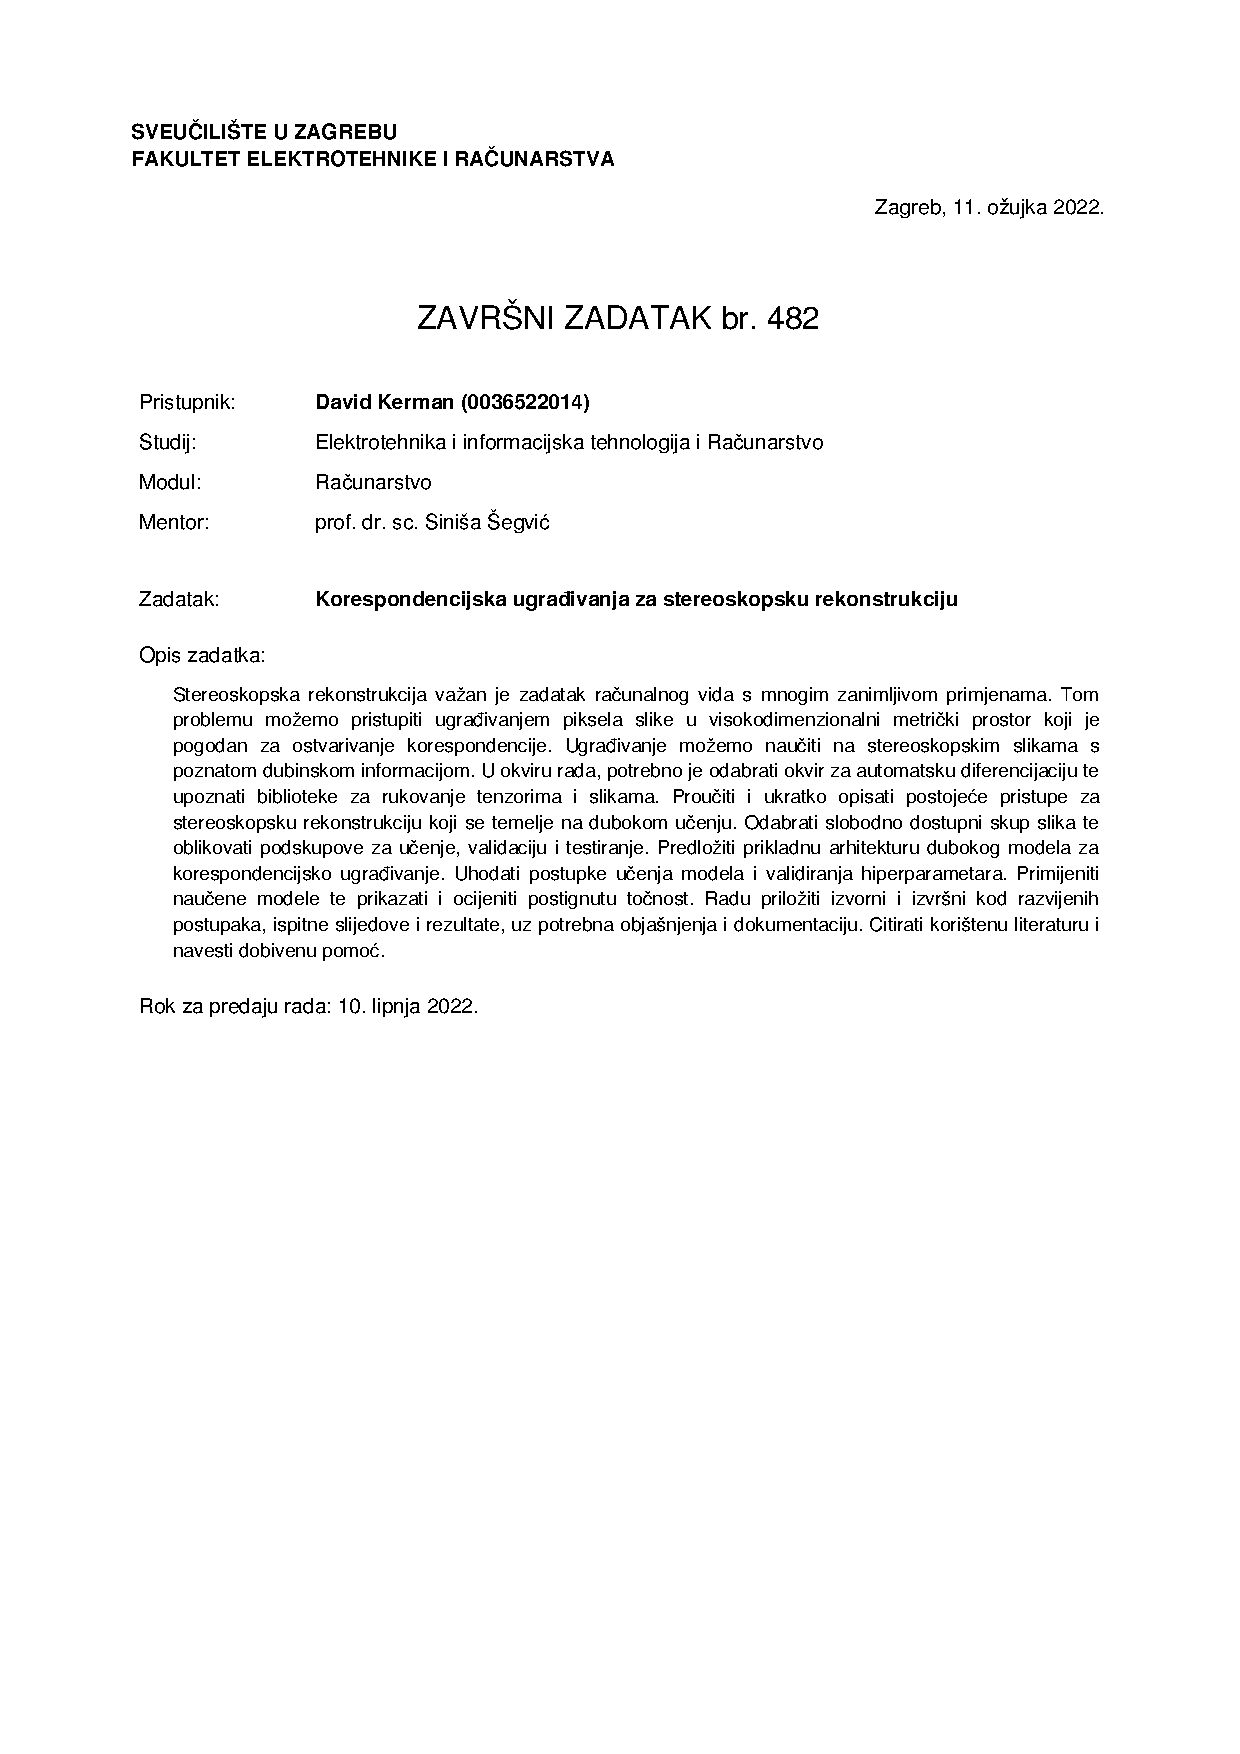
\includepdf[pages=-]{izvornik.pdf}

% Dodavanje zahvale ili prazne stranice. Ako ne želite dodati zahvalu, naredbu ostavite radi prazne stranice.
\zahvala{Zahvaljujem mentoru prof.~dr.~sc.~Siniši Šegviću, na savjetima i ukazanoj pomoći. Zahvaljujem kolegi Antoniu Ilinoviću na diskusijama i pomoći tijekom izrade rada. Također, zahvaljujem svojoj obitelji, prijateljima i kolegama na potpori tijekom mojeg dosadašnjeg obrazovanja.}

\tableofcontents

\chapter{Uvod}
Računalni vid kao jedna od temeljnih grana umjetne inteligencije omogućava računalima da izluče značajnu informaciju iz slika, videa ili sličnih vizualnih ulaza. Područje stereoskopske rekonstrukcije ima za cilj ostvariti stvaran trodimenzionalan položaj točaka koje su promatrane u dvije ili više slika, te kao takvo ima vrlo široke primjene uključujući one za određivanje sličnosti slikovnih okana. Kroz povijest postojale su klasične metode za određivanje korespodencijskih metrika, no pojavom snažnijih računala iskorišteno je duboko učenje kao alat kojim je moguće korespodencijske metrike naučiti na stvarnim podacima. Za potrebe metoda temeljenih na ugrađivanju u visokodimenzionalni prostor potrebne su rektificirane stereoskopske slike s poznatom dubinskom informacijom.\\

U okviru ovog radu opisana je geometrija stereoskopskog para, kalibracija, rektifikacija i algoritmi korišteni za ostvarivanje korespodencije. Zatim definirani su osnovni pojmovi u dubokom učenju, te postupci korišteni u dubokom učenju uz memorijske zahtjeve. Predstavljen je podatkovni skup na kojem su izvršeni postupci treniranja i validacije. Opisan je model kojim je ostvareno korespodencijsko ugrađivanje slikovnih okana, koji su korišteni u stereoskopskoj rekonstrukciji. Nastavno na to, opisan je postupak učenja takvog modela, te eksperimentalno vrednovanje rekonstrukcijske točnosti.

\chapter{Stereoskopska rekonstrukcija}
\section{Epipolarna geometrija}
Epipolarna geometrija je geometrija koja ima primjenu u stereoskopskoj rekonstrukciji, a po definiciji opisuje odnos točaka u slikama dobivenih iz dviju kamera. Također naziva se i epipolarno ograničenje jer uvelike smanjuje broj točaka koje je potrebno provjeriti pri traženju korespodentnih točaka. Točka $X$ koja je prikazana na slici 2.1 prikazuje točku u 3D prostoru koja se snima iz dviju kamera. Točke $C$ i $C'$ prikazuju centre lijeve, odnosno desne kamere. Projekcija točke $X$ na ravninu lijeve kamere je $x$, a na ravninu desne kamere $x'$. Važno je napomenuti da su točke $X$, $x$ i $x'$ u istoj ravnini, te zajedno sa centrima kamera $C$ i $C'$ čine tzv. \textit{epipolarnu ravninu} $\pi$.\\
\begin{figure}[htb]
\centering
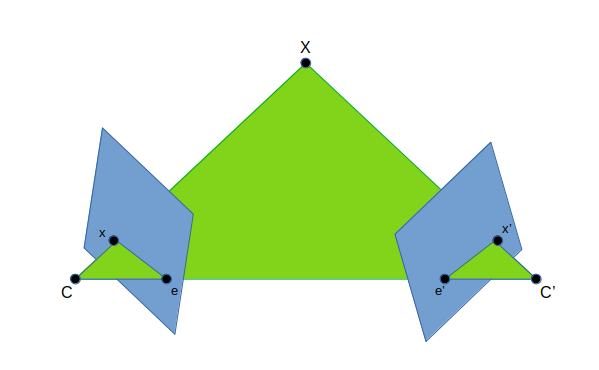
\includegraphics[scale=0.46]{img/slika1.png}
\caption{Epipolarna ravnina u kojoj se nalaze točka $X$,te točke nastale projekcijom $x$ i $x'$}
\label{fig:Epipolar}
\end{figure}\\
Nadalje, na slici su označeni \textit{epipolovi} oznakama $e$ i $e'$ te oni prikazuju točke u kojima pravac koji povezuje centre kamera $C$ i $C'$ siječe slikovne ravnine.
Najvažniji element su \textit{epipolarne linije}, označene dužinama koje spajaju $x$ i $e$, te $x'$ i $e'$, ali su zapravo pravci koji su nastali presjekom epipolarne ravnine sa slikovnom ravninom. Epipol je točka u kojoj se sijeku svi epipolarni pravci.\\
Poznavajući činjenicu da se točke nalaze u istoj ravnini, te ako znamo položaj točke $x$ možemo odrediti položaj točke $x'$. Rješenja koja se moraju ispitati da bi saznali položaj točke $x'$ nalaze se na epipolarnoj liniji, što uvelike olakšava pronalaženje korespodentnih točaka.

\section{Pretprocesiranje slika}
Parametre geometrije sustava kamera moguće je  podijeliti na dvije vrste: intrinzični i ekstrinzični. Ekstrinzični parametri su oni koji opisuju odnos svojstva koja su zajednička kamerama. Intrinzični pak opisuju svojstva kamera koje se odnose svaku kameru pojedinačno. Kao primjere za intrinzične faktore navodimo svojstva koja utječu na nji, a to su nesavršenost leća (na slici 2.2 prikazano je radijalno izobličenje), pomak senzora od centra leća te slične fizičke karakteristike nesavršenosti kamera.\\
\begin{figure}[htb]
\centering
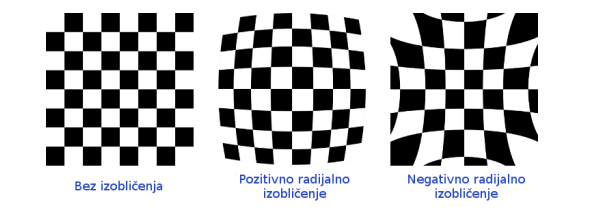
\includegraphics[scale=0.7]{img/slika2.png}
\caption{Primjeri radijalnog izobličenja. Izvor:\citep{bunjevac2017stereo}}
\label{fig:Radial}
\end{figure}\\
S druge strane ekstrinzični parametri nas dovode do nužnih transformacija kojima se slike dovode u istu ravninu projekcije te se time postiže da su pikseli duž horizontalnog pravca jedne slike na istoj visini na drugoj slici. Taj pravac je već spomenut, riječ je o epipolarnoj liniji. Ovakvim transformacijama uvelike se olakšava pronalaženje korespodentnih točaka koje u ovom slučaju treba tražiti samo duž jedne linije, epipolarne linije. Problem je sveden na jednu dimenziju. Kalibracijom se riješava problem nesavršenosti leća, odnosno problem izobličenja slika.\\
\\

\subsection{Rektifikacija}
Za postupak rektifikacije važni su ekstrinzični faktori kamera, dok na njihov izračun utječu intrinzični faktori. Transformacijom slika rektifikacijom dobivamo slike čiji pikseli koji u prostoru odgovaraju točkama na istoj visini,a nalaze se duž iste epipolarne linije. Također, nakon provedenih transformacija intrinzični parametri kamera postaju jednaki.\\
\begin{figure}[htb]
\centering
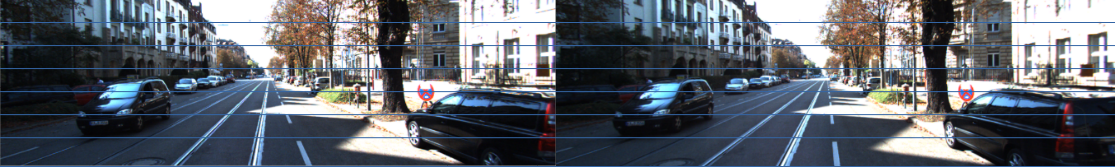
\includegraphics[width = 14.5cm]{img/slika3.png}
\caption{Prikaz epipolarnih linija u rektificiranim slikama skupa KITTI 2015}
\label{fig:Radial}
\end{figure}\\
Postupak se provodi kroz nekoliko koraka, a uključuje šahovsku ploču koja je pogodna zbog svojih svojstava. Prvi korak je traženje šahovskih polja. Postupak se nastavlja određivanjem izobličenja i ostalih parametara uz pomoć šahovskih polja.
Na slici 2.2 prikazan je par slika iz stereo kamera koji je rektificiran. Slike su iz skupa KITTI 2015, te se na njima vide epipolarne linije. Lako je primjetiti da iste točke u prostou nalaze na istoj visini, odnosno na istoj epipolarnoj liniji. Ovakvom transformacijom, korespodentne piksele potrebno je tražiti samo na istoj $y$-koordinati.

\section{Disparitet}
Prijašnjim postupcima kalibracije i rektifikacije omogućen je postupak računanja dispariteta, odnosno postupak računanja koji za svaki piksel koji je nastao lijevom kamerom određuje piksel slike koja je nastala desnom kamerom, ali pomaknutog za udaljenost $d$ piksela po horizonatlnoj osi. \textit{Disparitet} je definiran kao horizontalni pomak $d$ između dvaju korespodentnih piksela u slikama nastalim iz dviju konkurentnih stereo kamera. Kao rezultat računanja dispariteta nastaje mapa dispariteta koja sadrži disparitet za svaki piksel referentne kamere. Odnos piksela slike iz lijeve kamere, koja je u ovom slučaju referentna, i slike iz desne kamere definira se kao: 
\begin{equation}
I_{L}(x, y) = I_{D}(x-d,y)
\label{eq:Disparitet}
\end{equation}
gdje su $I_{L}$ i $I_{D}$ slike nastale lijevom, odnosno desnom kamerom, respektivno. Uređenim parom $(x,y)$ opisani su pikseli slike iz lijeve kamere, a njemu korespodentni pikseli u slikama iz desne kamere označeni su pomakom za disparitet $d$ po horizontalnoj osi $(x-d,y)$. Važno je napomenuti da su slike u skupu KITTI 2015 rektificirane i kalibrirane, što znači da korespodentne piksele tražimo samo po horizontalnoj osi.
Pomoću izračunatog dispariteta moguće je izraziti odnos između piksela kamera i dubine scene kao:
\begin{equation}
Z=f\frac{B}{d}
\label{eq:Fokalna}
\end{equation}
gdje je dubina scene, odnosno udaljenost objekta od kamere označena sa $Z$, $d$ je disparitet,s $B$ je označnena udaljenost između središta kamera, a s $f$ je označena fokalna udaljenost kamere. Iz jednadžbe 2.2 je vidljiva obrnuta proporcionalnost između udaljenosti objekta od kamera, te dispariteta s druge strane. Kada je položaj objekta blizu kamere, disparitet će biti velik. A kako se udaljavamo od kamere, disparitet se smanjuje i u beskonačnosti postiže vrijednost 0.\\
Na slici 2.4. je vidljivo da su epipolarne linije paralelne, te im je $y$-koordinata za korespodentne piksele jednaka. Disparitet je označen slovom $d$ i prikazuje horizontalni pomak.
\begin{figure}[htb]
\centering
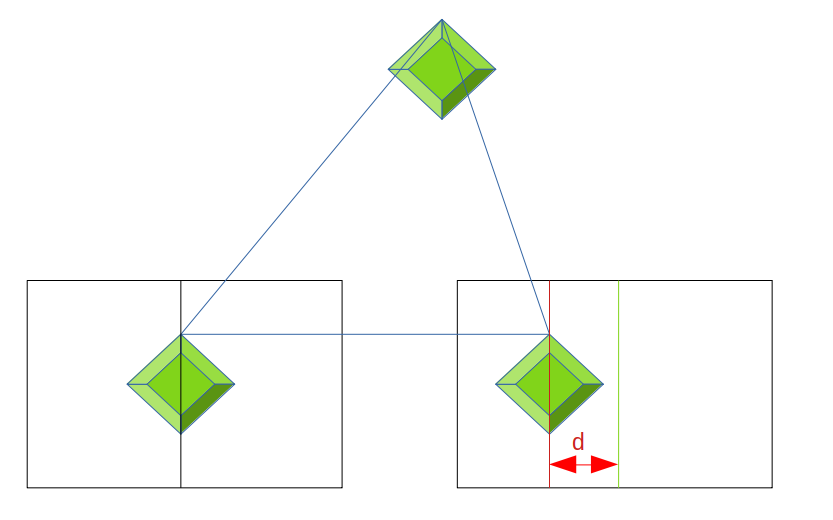
\includegraphics[width = 14.5cm]{img/slika4.png}
\caption{Prikaz objekta u slikama iz lijeve i desne kamere. Plavom bojom označena je epipolarna ravnina. Okomitim osima označeni su projicirani pikseli u konkuretnim slikama. Disparitet je označen slovom $d$.}
\label{fig:Disparitet i epipolar}
\end{figure}\\
\\\\
\section{Algoritam stereoskopske rekonstrukcije}
Postupak stereoskopske korespodencije je zapravo postupak pronalaženja istih piksela u međusobno konkurentnim kamerama koji odgovaraju istoj točki u trodimenzionalnom prostoru. Postoje dvije vrste korespodencija, \textit{rijetke} i \textit{guste}. Razlika je u tome što rijetke ne izračunavaju disparitete za sve piksele, dok guste to rade. Guste korespodencije omogućene su današnjom snagom računala, te se rijetke više toliko ne koriste. Postupak guste korespodencije je tim teži što se prilikom izračuna susreće s nekim anomalijama u slikama, primjerice područjima bez teksture, reflesivnim podlogama na kojima se svjetlost drugačije lomi i odbija, te točkama koje se iz jedne kamere vide, a iz druge ne (\textit{stereoskopska sjena}).\\
Dolazimo do stereo algoritama, svaki od njih moguće je opisati u četiri koraka (\citep{scharszelinski}, \citep{kovac2015stereo}):
\begin{enumerate}
\item izračunavanje razlike između dvaju slikovnih okana, odnosno izračun podatkovnih cijena po prije definiranoj mjeri razlike
\item prikupljanje podatkovnih cijena za disparitete koji se razmatraju
\item izračun mape dispariteta, odnosno odabir najmanje prikupljene cijene za svaki piksel, uz optimizaciju
\item zaglađivanje mape dispariteta 
\end{enumerate}

Prvi korak ovog generičkog algoritma za stereoskopsku rekonstrukciju je izračun podatkovnih cijena. Izračun podatkovnih cijena može se računati prema pojedinačnim pikselima ili skupini piksela.  Izračun nam govori kolika je razlika između dvaju slikovnim okana, a razlika koja se koristi je definirana prije. Mjere razlike mogu biti sljedeće:
\begin{itemize}
\item[•] srednja kvadratna razlika
\item[•] srednja apsolutna razlika
\item[•] kvadratna razlika između intenziteta piksela
\item[•] apsolutna razlika između intenziteta piksela
\end{itemize}

\newpage
Drugi od koraka generičkog stereo algoritma je prikupljanje podatkovni cijena, tj. agregacija.  Na početku je postavljena granica za maksimalan disparitet, pa se tijekom ovogg koraka izračunava podatkovna cijena za sve disparitete i skupa  od $0$ do $D$, te ćemo tako za svaki piksel imati $D+1$ podatkovnih cijena.\\
Treći korak algoritma je izračun mape dispariteta. Nakon što su izračunate podatkovne cijene za razmatran skup dispariteta, treba odabrati metodu za izračun mape dispariteta. U praksi postoje \textit{lokalne} i \textit{globalne}. Lokalne metode prikupljaju cijene nad ograničenim područjem unutar same mape dispariteta, odnosno traže na ograničenom području oko referentne točke. Područje moje biti 2D ili 3D, te se prikupljanje može primjerice izvesti konvolucijom. S druge strane, globalne metode  preskaču korak prikupljanja podatkovnih cijena, te odmah nakon izračuna podatkovnih cijena vrše optimizaciju. Globalne metode minimiziraju kriterij nad cijelom slikom. Odnos između ovi metoda može se svesti na to da su lokalne brže, no globalne daju puno glađe mape dispariteta, što ih čini kvalitetnijima.\\
Zadnji korak koji je naveden je zaglađivanje mapa dispariteta. Ovaj korak je opcionalan i neke metode ga koriste. Glavni cilj ovog koraka je uklanjanje šuma koji je nastao generiranjem mape. 
\chapter{Duboko učenje}
Duboko učenje grana strojnog učenja koje se ubrzano razvija. U teoriji se dubokim učenjem smatra proces učenja neuronske mreže s 3 ili više slojeva, sve što je manje od toga naziva se \textit{plitkim} modelima. Cilj takvih neuronskih mreža je simulirati ponašanje ljudskog mozga omogućujući učenje na velikim skupovima podataka. Zahvaljujući razvoju grafičkih kartica, omogućen je ubrzan razvoj dubokog učenja.

U sljedećim odjeljcima bit će predstavljeni osnovni pojmovi i koncepti korišteni prilikom oblikovanja modela i procesa učenja.
\section{Osnovni pojmovi u dubokom učenju}
\subsection{Perceptron}
U ranim počecima duboko učenja došlo se do ideje potpuno povezanih modela. Jedan od takvih modela je višeslojni perceptron. Iako je danas napuštena ideja potpuno povezanih modela, zanimljivo je pogledati koje mane novi modeli imaju za ispraviti.
\begin{figure}[htb]
\centering
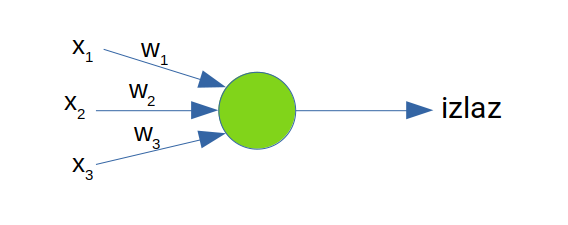
\includegraphics[width = 14.5cm]{img/slika5.png}
\caption{Jednostavni perceptron}
\label{fig:Perceptron}
\end{figure}
\newpage
Perceptron je prvi definirao Frank Rosenblatt. Na slici 3.1. prikazan je jednostavni perceptron. Perceptron ima više binarnih ulaza koji su označeni s $x_{1}$, $x_{2}$ i $x_{3}$, te proizvodi binarni izlaz. Rosenblatt je, kako bi odredio izlaz, definirao težine (u ovom slučaju $w_{1}$, $w_{2}$ i $w_{3}$). Težinama se mogu opisati doprinosi jednog neuorona na drugi, odnosno koliko jedan utječe na drugog. Ovime je izlaz neurona definiran sumom umnoška težina i binarnih ulaza te praga s kojim s uspoređuje:
\begin{subequations}
\begin{empheq}[left=\ \empheqlbrace]{align}
0, {\sum_{k=1}^{n}} w_kx_k \le prag \\
1,  {\sum_{k=1}^{n}} w_kx_k > {prag}
\end{empheq}
\label{eq:Perceptron}
\end{subequations}
Jedan sloj neuronske mreže čine perceptroni koji se nalaze u istom stupcu. Izlaz svakog perceptrona  izračunava se tako koristeći izlaze prethodnog sloja i definirane težine za svaki od ulaznih perceptrona. Gornju formulu moguće je transformirati tako što se prag uvede nova varijabla $b=-prag$, koja označava pristranost (engl. \textit{bias}). Pristranost u kontekstu duboko učenja je moguće definirati koliko je lako natjerati neuron  da kao izlaz izbaci 1. Ukoliko je pristranost vrlo velik broj, izlaz e u veini slučajeva biti 1, dok je za vrlo negativan broj suprotna situacija. Izmijenjena formula glasi:
\begin{subequations}
\begin{empheq}[left=\ \empheqlbrace]{align}
0, {\sum_{k=1}^{n}} w_kx_k  + b\le 0 \\
1,  {\sum_{k=1}^{n}} w_kx_k + b > 0
\end{empheq}
\label{eq:Perceptron}
\end{subequations}
Linearnu funkciju koju smo izveli možemo predstaviti i u matričnom obliku:
\begin{equation}
f=w^{T}x+b
\label{eq:Linear}
\end{equation}
\subsection{Prijenosne funkcije}
Ukoliko bi koristili linearnu funkciju izlaza iz prijašnjeg odjeljka, mala promjena u ulazu bi na izlazu generirala veliku promjenu. Stoga se uvode prijenosne, odnosno aktivacijske funkcije jer odlučuju hoće li neki neuron biti aktivan ili ne. Primarni cilj prijenosnih funkcija je omogućiti da se primijete sitne promjene na ulazu. Aktivaciju neurona možemo predstaviti sljedećom formulom:
\begin{equation}
a^k=\sigma_{k}(W^T_{k}a^{k-1}+b)
\label{eq:Aktivacija}
\end{equation}
gdje $a^k$ označava aktivaciju neurona trenutnog sloja, $a^{k-1}$ aktivaciju neurona prijašnjeg sloja, dok $\sigma$ označava aktivacijsku funkciju.

Prva funkcija koja će biti objašnjena je sigmoidalna funkcija čiji izraz je dan u nastavku:
\begin{equation}
\sigma(x)=\frac{1}{1 + e^{-x}}
\label{eq:Aktivacija}
\end{equation}
Glavno obilježje sigmoidalne funkcije je to što je njezina kodomena na skupu od 0 do 1, te ju to čini primjenjivom u regresijskim i klasifikacijskim problemima. Veliki pozitivni brojevi poprimit će vrijednost 1, dok će jako negativni brojevi poprimiti vrijednost 0. Također, prednost je što je derivabilna, pa omogućuje učenje u kojem se koristi gradijentni spust. Glavni nedostatak zbog kojeg se sve manje koristi je problem nestanja gradijenata (engl. \textit{vanishing gradient problem}) koji govori da gradijenti postaju toliko mali da ne nose nikakvu informaciju koja bi se mogla iskoristiti za učenje. Prikaz grafa funkcije je na slici 3.2.\\
\begin{figure}[htb]
\centering
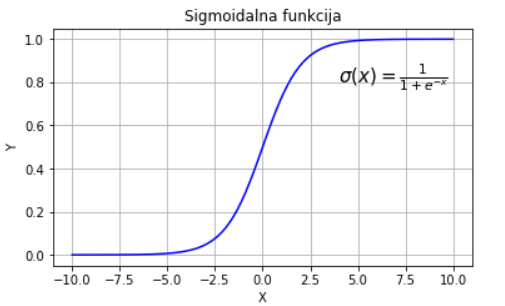
\includegraphics[scale=0.6]{img/slika6.png}
\caption{Graf sigmoidalne funkcije}
\label{fig:Perceptron}
\end{figure}
\linebreak
Funkcija koja je usko vezana uz sigmoidalnu je \textit{tangens hiperbolni}. Kodomena ove funkcije je na intervalu od -1 do 1. Problem nestajanja gradijenata je isto tako prisutan. Kako je bliska sigmoidalnoj, možemo uspostaviti odnos između njih koji je oblika:
\begin{equation}
\tanh(x) = 2\sigma(2x)-1
\label{eq:Aktivacija}
\end{equation}
\begin{figure}[htb]
\centering
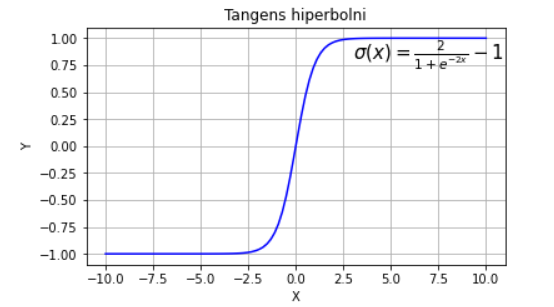
\includegraphics[scale=0.6]{img/slika7.png}
\caption{Graf funkcije tangensa hiperbolnog}
\label{fig:Perceptron}
\end{figure}\\
\\\\\\\\
Sljedeća prijenosna funkcija koja se koristi je zglobnica (engl. \textit{ReLU - rectified linear unit}). Ova prijenosna funkcija propušta pozitivne vrijednosti, dok negativne vrijednosti ne propušta. Glavna prednost ove funkcije što je računski izuzetno jeftina, dok joj je nedostatak što za negativne vrijednosti uvijek daje 0. Izraz koji ju opisuje je oblika:
\begin{equation}
f(x)=max(0,x)
\label{eq:Aktivacija}
\end{equation}
\begin{figure}[htb]
\centering
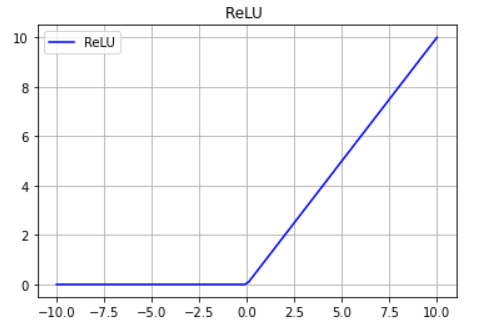
\includegraphics[scale=0.6]{img/slika8.png}
\caption{Graf funkcije ReLU}
\label{fig:Perceptron}
\end{figure}
\linebreak
\\\\
Moguće je napraviti modifikaciju zglobnice tako da za negativne vrijednosti daje vrlo male vrijednosti, te se takva prijenosna funkcija naziva propusnom zglobnicom (engl. \textit{LReLU - leaky rectified linear unit}). U nastavku slijedi izraz koji ju opisuje:
\begin{subequations}
\begin{empheq}[left={f(x)=}\ \empheqlbrace]{align}
x, x > 0 \\
\alpha x,  x \le 0
\end{empheq}
\label{eq:Perceptron}
\end{subequations}
gdje je $\alpha$ parametar, odnosno u praksi vrlo mali pozitivan broj. Na slici 3.5. je vidljivo da negativne vrijednosti propušta uz prigušenje, dok na slici 3.4. obična zglobnica ne propušta.
\begin{figure}[htb]
\centering
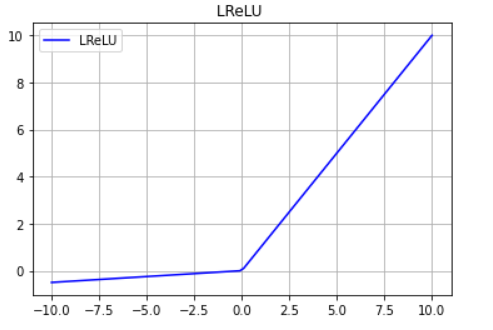
\includegraphics[scale=0.6]{img/slika9.png}
\caption{Graf funkcije LReLU}
\label{fig:Perceptron}
\end{figure}
\subsection{Konvolucijski slojevi}
Konvolucijski slojevi osnovni su gradivni element konvolucijskih neuronskih mreža. Kako je u radu riječ o slikama, bit će predstavljena $2D$ konvolucija, operacija filtriranja. Uloga filtriranja je uočavanje i učenje uzoraka koji se nalaze na slikama. 
Konvolucijski slojevi čine konvolucije ulaza s različitim filtrima, drugi naziv je jezgra (engl. \textit{kernel}).Izlaz iz 2D konvolucije je aktivacijska mapa, odnosno mapa značajki, dok je izlaz cijelog konvolucijskog sloja više mapa značajki. Kako dubina tijekom prolaska kroz mrežu raste, identificiraju se sve specifičniji uzorci. Tijekom unaprijednog prolaza, jezgra se provlači po matričnoj reprezentaciji slike i računa se skalarni umnožak između jezgre i ulaza na svakom položaju. 
\\\\\\
\begin{equation}
\begin{bmatrix}
x_{11} & x_{12} & x_{13} \\
x_{21} & x_{22} & x_{23} \\ 
x_{31} & x_{32} & x_{33}
\end{bmatrix}*\begin{bmatrix}
w_{11} & w_{12} \\
w_{21} & w_{22}
\end{bmatrix}=
\begin{bmatrix}
x_{11}w_{11} + x_{12}w_{12} & x_{12}w_{11} + x_{13}w_{12}\\+ x_{21}w_{21} + x_{22}w_{22} &   + x_{22}w_{21} + x_{23}w_{22}\\ 
\\
x_{21}w_{11} + x_{22}w_{12} & x_{22}w_{11} + x_{23}w_{12}\\+ x_{31}w_{21} + x_{32}w_{22} &  +x_{32}w_{21} + x_{33}w_{22}
\end{bmatrix}
\label{eq:Aktivacija}
\end{equation}
\linebreak
Jednadžbom 3.9 prikazana je matrična reprezentacija dimenzija $3x3$, dok je jezgra dimenzije $2x2$. Jezgra se provlači po ulaznoj matrici (računa se skalarni umnožak) i nastaje izlazna mapa značajki dimenzija $2x2$. Iz ovog je vidljivo da se konvolucijom smanjuje dimenzija ulaza.

Ukoliko želimo zadržati rezoluciju slike nakon konvolucijskog sloja, potrebno je uvesti nadopunjavanje (engl. \textit{padding}). Najčešće je korištena metoda popunjavanja nulama. Još jedan od hiperparametara je korak (engl. \textit{stride}). Korak govori o tome koliko se jezgra pomiče u vertikalnom i horizontalnom smjeru. U jednadžbi 3.9 je korišten korak 1.
\section{Učenje dubokih modela}
Učenje dubokih modela, u generalnom slučaju neuronske mreže, je postupak tijekom koje se modelu na ulaz daju podaci iz skupa za učenje. Tijekom procesa učenja model ažurira težine u slojevima s ciljem kako bi što bolje aproksimirao izlaznu funkciju. Za početak kako bi mogli odrediti koliko odstupamo od pravih vrijednosti, uvodimo pojam funkcije gubitka. U procesu učenja provodi se minimizacija funkcije gubitka. Ukoliko na skupu podataka gubitak ispada malen, a na skupu podataka koje još nije vidio ispada izražen, govorimo o tzv. prenaučenosti modela, što znači da model nema sposobnost generalizacije.\\
Postoji nekoliko pristupa učenju, nadzirano učenje u kojem se modelu predaju parovi oblika (ulaz, željeni izlaz), nenadzirano u kojem se modelu samo predaju ulazni podaci, te podržano učenje u kojem se maksimizira kumulativna nagrada. U ovom radu bit će razmatrano nadzirano učenje.\pagebreak
\subsection{Funkcija gubitka}
Kako bismo procijenili koliko model odstupa od željenih vrijednosti izlaza koristimo funkciju gubitka. Ako model loše procjenjuje, gubitak će biti velik. 
Kod problema klasifikacije najčešće je korištena unakrsna entropija (engl.\textit{cross-entropy loss}):
\begin{equation}
L_{CE}=-\sum_{i=1}^{n}t_{i}\cdot log(p_{i})
\label{eq:Aktivacija}
\end{equation}
Popularan klasifikator koji koristi unakrsnu entropiju, a daje vjerojatnosnu reprezentaciju izlaza modela je funkcija \textit{softmax}:
\begin{equation}
f_{j}(z) = \frac{e^{{z_{j}}}}{\sum_{k}^{}e^{z_{k}}}
\label{eq:Aktivacija}
\end{equation}
\subsection{Gradijentni spust}
U prijašnjem pododjeljku definirana je funkcija gubitka, cilj učenja modela je minimizirati gubitak. Kako bi se parametri pomicali u smjeru minimuma funkcije gubitka, a da istovremeno pomak bude što veći izračunava se gradijent funkcije gubitka. \\
Neka je zadana funkcija gubitka koja ovisi o težinama $\textbf{W}$ i pomacima $\textbf{b}$. Gradijenti funkcije gubitka mogu se zapisati kao:
\begin{equation}
\nabla L_{w} = \left(\frac{\partial L}{\partial w_{1}},...,\frac{\partial L}{\partial w_{n}} \right)
\label{eq:Aktivacija}
\end{equation}
\begin{equation}
\nabla L_{b} = \left(\frac{\partial L}{\partial b_{1}},...,\frac{\partial L}{\partial b_{n}} \right)
\label{eq:Aktivacija}
\end{equation}
gdje $n$ predstavlja broj parametara.\\
U iteracijama gradijentnog spusta parametri se ažuriraju prema sljedećim izrazima:
\begin{equation}
W_{i+1} = W_{i} - \epsilon \cdot \nabla L_{w}(\textbf{W},\textbf{b})
\label{eq:Aktivacija}
\end{equation}
\begin{equation}
b_{i+1} = b_{i} - \epsilon \cdot \nabla L_{b}(\textbf{W},\textbf{b})
\label{eq:Aktivacija}
\end{equation}
gdje je $\epsilon$ tzv. stopa učenja (engl. \textit{learning rate}), a predstavljena je malim pozitivnim realnim brojem.\cite{duboko} \pagebreak
\subsection{Optimizacija}
Kad govorimo o optimizaciji, najkorištenija metoda je svakako gradijentni spust, no korištenjem njega se mogu manifestirati neki problemi koji kao posljedicu imaju nepronalazak optimalnih težina. Postojanje više lokalnih minimuma i spora kovergencija jedni su od problema. 
U ovom radu je korišten ADAM optimizator,a svakako potrebno je spomenuti i SGD optimizator. 

Glavna ideja optimizatora SGD je procijeniti gradijent cijelog skupa uzoraka sa malim slučajno odabranim podskupom uzoraka (mini-grupa, engl. \textit{minibatch}). Već i veličine od 128 daju vrlo dobru aproksimaciju gradijenta. U usporedbi s "običnim" gradijentnim spustom (GD) to znatno ubrzava proces učenja, jer se kod GD izračun treba provesti za cijeli skup. Stohastički gradijentni spust koristi se uz zalet koji ubrzava učenje. Umjesto ažuriranja težina koristeći samo trenutno izačunat gradijent, zalet također uzima u obzir i prethodno ažuriranje, pomnoženo sa faktorom umanjivanja $\alpha$.\cite{sgd}\\ 
Modifikacija u odnosu na GD je vidljiva sljedećom jednadžbom:
\begin{align}
v = \mu v + \nabla L_{w}
\end{align}
,gdje je $v$ trenutno akumuliran zalet, a $\mu$ je zalet.

Adaptive Moment Estimation (ADAM) je optimizator koji kombinacijom dvije metodologije gradijentnog spusta zaleta i RMSprop algoritma ubrzava pronalazak globalnog minimuma. Glavna značajka ADAM-a je što koristi prosječno eksponencijalno kretanje gradijenta i kvadratnog gradijenta, te ga to čini izrazito efikasnim na velikim skupovima podataka i u radu s velikim brojem parametara\cite{adam}.
\subsection{Regularizacija}
Kako bi se izbjegla prenaučenost modela (engl. overfitting), odnosno loša generalizacija modela potrebno je uvesti regularizatore koji imaju za cilj spriječiti prenaučenost.\\
Jedna od metoda koje se koriste je regularizacija dodavanjem regularizacijskog faktora funkciji gubitka. Pri tome treba spomenuti $L1$ i $L2$ regularizaciju, kojima se kažnjava norma vektora težina.
\begin{equation}
L_{R}= L + \lambda \cdot \sum_{i} |w_{i}|
\label{eq:Aktivacija}
\end{equation}
\begin{equation}
L_{R}= L + \lambda \cdot \sum_{i} w_{i}^2
\label{eq:Aktivacija}
\end{equation}
Izrazom 3.17 opisana je $L1$ regularizacija, a 3.18 $L2$ regularizacija.\\ \\
Regularizacijska metoda koja istovremeno ima i ulogu optimizacije je normalizacija grupe (engl. \textit{batch norm}). Normalizacija grupe primjenjuje se prije nelinearnosti, a temelji se na normalizaciji izlaza na normalnu jediničnu razdiobu. Posljedica takvog pristupa je što ulazi u slojeve imaju sličnu razdiobu, čime se postiže ubrzanje učenja bržom propagacijom gradijenata.
U postupku normalizacije u mini grupi za svaku izlaznu mapu značajki računaju se srednja vrijednost i varijanca po sljedećim izrazima:
\begin{equation}
\mu _{B} = \frac{1}{m}\sum_{i=1}^{m}\textbf{x}_{i}
\label{eq:Aktivacija}
\end{equation}
\begin{equation}
\sigma^{2} _{B} = \frac{1}{m}\sum_{i=1}^{m}\left(\textbf{x}_{i} - \mu_{B} \right)
\label{eq:Aktivacija}
\end{equation}
gdje $B$ označava mini grupu, a $x$ vrijednost ulaza.
Nelinearnost se onda primijenjuje na tako normaliziranom izlazu.
\chapter{Podatkovni skup za učenje}
Kako je već rečeno, u ovom radu učenje je nadzirano. Podatkovni skup KITTI jedan je od skupova koji se koriste u učenju postupka stereoskopske rekonstrukcije.U sljedećem pododjeljku bit će predstavljen podatkovni skup KITTI 2015, njegove specifičnosti, te postupci pripreme podataka.
\section{Podatkovni skup KITTI 2015}
Podatkovni skup KITTI 2015, skup je od 200 stereo parova slika za koje su laserski izmjerene mape dispariteta. Stereo par slika je unaprijed kalibriran i rektificiran. Primjer uz odgovarajuće disparitete prikazan je na slici 4.1. Podatkovni skup je često korišten u postupcima stereoskopske rekonstrukcije za autonomnu vožnju.Podatkovni skup je podijeljen na skup za učenje kojeg čini 60\% slika, sljedećih 20\% čini skup za validaciju, te preostalih 20\% čini skup za testiranje.\\
Mape dispariteta su vrlo rijetke, odnosno dispariteti su izmjereni laserski za manji podskup piksela. Takve mape će na mjestima piksela za koje nije izmjeren disparitet imati vrijednost nula. Primjer takvih piksela su oni koji prikazuju udaljene objekte, kao što je nebo. Takvo mjerenje proizlazi iz toga što je disparitet obrnuto proporcionalan udaljenosti, te poprima vrijednost nula u beskonačnosti. \\
Također napravljena je intervencija na područjima slike na kojima se nalazi automobil. Intervencija se sastojala od progušćivanja dispariteta na mjestima automobila. Ova intervencija je od velike važnosti rekostrukcijskim algoritmima jer se na automobilu nalaze refleksivne površine poput stakla koje u konkurentnim stereo kamerama mogu izgledati drugačije.\cite{zbontar}
\begin{figure}[htb]
\centering
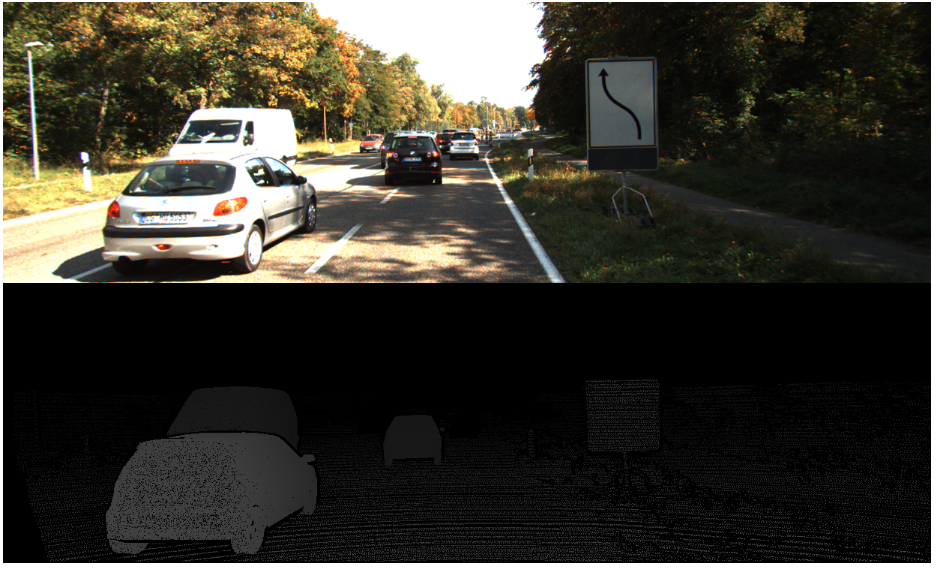
\includegraphics[width = 14.5cm]{img/slika11.png}
\caption{Primjer iz podatkovnog skupa KITTI 2015. Gornja slika prikazuje referentnu lijevu sliku, a donja slika prikazuje disparitet za odgovarajuću sliku.}
\label{fig:KITTI}
\end{figure}
\chapter{Duboko učenje u kontekstu stereoskopske rekonstrukcije}
\section{Ugrađivanje okana u metrički prostor}
\section{Učenje modela za ostvarivanje korespodencije}
\chapter{Eksperimentalni rezultati}
\chapter{Programska izvedba i vanjske biblioteke}
\chapter{Zaključak}

\bibliographystyle{fer}
\bibliography{literatura}


\begin{sazetak}
Sažetak na hrvatskom jeziku.

\kljucnerijeci{Ključne riječi, odvojene zarezima.}
\end{sazetak}

% TODO: Navedite naslov na engleskom jeziku.
\engtitle{Title}
\begin{abstract}
Abstract.

\keywords{Keywords.}
\end{abstract}

\end{document}
